\section{Background}
\subsection{Biology}
cite(Tihanyi et al.):
Recombinant proteions are the proteins that are spreadly used in the biomedical research, medicine production and simply for many different therapeutic needs like vaccines or antibodies. Currently there is a great need for production of recombinant proteins in hight volumetric amounts and of a good quality. They are mostly produced from the mammalian cells namely Chinese hamster ovary cells (CHO). (doi:10.1016/B978-0-08-100623-8.00007-4) The process that is used for this production is called cell line development(CLD). And the current goal in recombinant protein production is to create a an efficient expression system and high-throughput systems to improve the CLD processes. (cite! Tihanyi et al.). 

CLD is a process of generating single cell-derived clones that produce high and consistent levels of target therapeutic protein. (pharma.lonza.com/offerings/mammalian/cell-line-development)


There are many different proteins that can be produced using such technologies, for ex. vaccines, hormones, sugars and etc., however this research is dedicated to the production of monoclonal antibodies (mAbs). 

The reason behind the use of mammalian cells hides in the fact that they can produce diverse correctly folded proteins and most importantly they have a high productivity. (cite Tihanyi). The productivity is measured in titre of the produced protein, and they can reach (0.1 - 1 g/L in batch and 1-10 g/L in fed-batch cultures). (cite Tihanyi TODO explain batch) Mostly all of the mAbs are produced using CHO cells (cite http://dx.doi.org/ 10.1016/j.jbiotec.2017.04.028.).

Currently companies use the same host cell line for their productions as well as in clinical trials as already checked and qualified cells simplify their road to the clinic. Therefore current reasearch can have a wide applicability in all CHO protein productions.

However there is a downside in the use of CHO cells as they are well-known by their instability. As a rapidly growing immortal cells they are also genomically unstable and extremely heterogeous which ususally leads to their mein problem - production instability. The problem of choosing the stable and high producing clones that also will be able to also express protein quailitatively and quantitably over time is essentially the main problem which is solved in this research.

The main problems for manufacturing is of course the cost and times of productions. Right now most of the research attention is dedicated to the the reduction of the time and costs for CLD processes, as well as for developing techniques of high-throughput clone screening and characterization. (cite Tihanyi). With the great amounts of data acquired over time and the development of the computational modelling and statistical analysis it is possible now to do the analysis \textit{in silico}, meaning - computationally without intervening into the cells instead of the usual \textit{in vitro} analysis.

Differential interference contrast (DIC) microscopy is an optical microscopy technique used to enhance the contrast in unstained, transparent samples (wikipedia).

Proteins are large biomolecules and macromolecules that comprise one or more long chains of amino acid residues (https://en.wikipedia.org/wiki/Protein).

Fluorescent labelling is the process of covalently binding fluorescent dyes to biomolecules such as nucleic acids or proteins so that they can be visualized by fluorescence imaging (https://www.nature.com/subjects/fluorescent-labelling). A fluorophore is a chemical compound that can reemit light at a certain wavelength.These compounds are a critical tool in biology because they allow experimentalists toimage particular components of a given cell in detail. (O'reilly life sciences p113)

Cell line development (CLD) is the process by which the cellular machinery is co-opted to manufacture therapeutic biologics or other proteins of interest. One can use different expression systems for cell line development: bacterial, plant-based, yeast, mammalian. (copy paste from https://www.beckman.de/resources/product-applications/lead-optimization/cell-line-development)


First step of CLD is the
introduction of the gene of interest (GOI or a DNA vector or an expression vector) to CHO cells. This process is called a transfection. And it has two main downsides: first is that the transfection mostly results in a vector being inserted into a random site within a host cell genome and second, generally low efficiency of integration (cite Tihanyi). It is important to transfect a GOI into an optimal site of genome to secure a high protein expression over time during protein production, however pratically transfection. In case the gene was transfected in the inactive site of genome (and the majority of genome is not transriptionally active) the cell will likely not express the gene. (doi:10.1016/B978-0-08-100623-8.00007-4) (doi:10.1016/j.coche.2018.08.002)

The second step is the selection of cell pools that have successful and stable gene integrations. The reasond why not all of them are suitable for cloning is the following: during the transfection only 80\% of cells recieve the vector of GOI (doi:10.1016/B978-0-08-100623-8.00007-4), only the small percent of which actually integrate a vector into the genome and, as mentioned above, only a fraction of those cells are able to stabily express a protein. (Reference needed). Such selection could be done with bulk sorting algorithm. (doi:10.1016/B978-0-08-100623-8.00007-4)

The third step in CLD is to clone the cells. The chosen stable pools of cells are phenotypically and genetically diverse - meaning they have different growth rates, metabolic profile and etc. This is not ideal for industrial production - all the cells used for protein production should be derived from the same clone ([25] here doi:10.1016/B978-0-08-100623-8.00007-4). In order to choose single best cells for further cloning one asseses several parameters like cell size, granularity, cell surface protein expression and etc. This can be done with Fluorescent Activated Cell Sorting (FACS) technology that allows to sort signle cells. (https://doi.org/10.1517/14712598.4.11.1821). Unfortunately fluorescence labeling is expensive and may ruin the cell due to its phototoxicity (https://doi.org/10.1371/journal.pone.0007497). Yeo et al. (cite Tihanyi) also found out how different selection markers can affect the production stability of CHO cells. There is a limited number of available fluorescent channels in microscopes as well as such labels can also be inconsistent, depend a lot on reagent quality, and require many hours of lab work. Therefore there exists a need for flurescent labeling in silico - without intervening into the cell. 

Assessing the productivity rates of the clones is very labour intensive and time-consuming process that can and should be optimized.

Once the cells are cloned, phenotypical and genetical heterogeneity is reduced, the next step is to charaterize clonally-derived cells based on the following criteria: cell size, growth rate, protein quality, titer, metabolities and etc. With this one can estimate clones productivity and titer. Such observations may take up to 90 days after which one can determine which cells are stable and therefore suitable for production. This is the last step of CLD process and consumes a lot of time and maintaining costs for feeding and cloning the cells. Predicting the stability of the cells directly from DIC images would reduce this time significantly allowing to escape this process completely.

However there are also some disadtantages of this approach. First, it can be less accurate than skilled cells staining perfomed manually. Extreme or unsual clones and phenotypes might be challenging if they were not used in the training set of images.

\subsection{Imaging}
The microscope used in the experiments takes photos of the well plate in random locations. The reason for that hides in the focusing problem, to get a reasonably good photo without blur it has to focus on a specific location, this is done there automatically, therefore the location of the focus is almost random (see Figure \ref{fig:random-dic}). 

\begin{figure}[htb]
	\begin{center}
		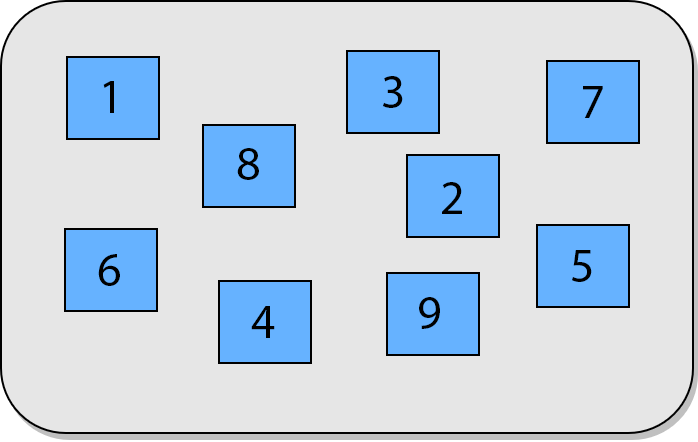
\includegraphics[width=0.5\linewidth]{bilder/dic-random.png}
		\caption{Way in which photos of the well-plate were taken}\label{fig:random-dic}
	\end{center}
\end{figure}


Although it might be problematic in the following sense: photos takes by the microscope in such manner do not gurantee that the focus will land in distinct spots all the time. This means that some cells taken during one of the photos might appear in the later ones. Since the photos have a high-resolution the crops are first performed and it might happen that same cell might appear in several crops. Afterwards, when crops are split between train, test and validation datasets it might happen that the same cell will once land in the train set and another time in the validation set, which will lead to a not completely fair and representative validaiton loss during training.

\subsection{ML}
Background on Unet and ML in general

Convoutional neural network is a neural network that is based on convolutional layers. It is a powerful tool for image processing and is used in medical imaging. Convolution is a linear operation used in convolutional layers that can be performed by applying a kernel (a 2d matrix) across a bigger input matrix called tensor, which can be 3d. Element-wise product between them is calculated and summed, this value will be an element of the output 2d matrix. Kernel slides accross all locations of the input tensor. In case if several different kernels were used then a 3d tensor will be created. 

Main advantage of convolutional neural networks if weight sharing. Kernel has learnable weights however these weights are shared across all locations of the kernel on the input tensor, thic strongly reduces the number of parameters needed.

CNNs also uses non-linearities like RELU, ELU, Tahn, Sigmoids and etc. They are also often combined with max pooling layers and dropouts to escape overfitting. 

Overfitting is one of the most often problems in deep learning that prevents model to generalize well for unseen data. This can happen when the model is too big for the amount of training data given, it was not regularized well or there is just not enough data for training. 

U-Net architecture is widely used for segmentation purposes. It is a convolutional neural network with the following architecture: [img] . It first performs image downsampling and upsampling afterwards.
[https://arxiv.org/pdf/1505.04597.pdf] The following architecture have been used for nuclei prediction. 
\begin{figure}[htb]
	\begin{center}
		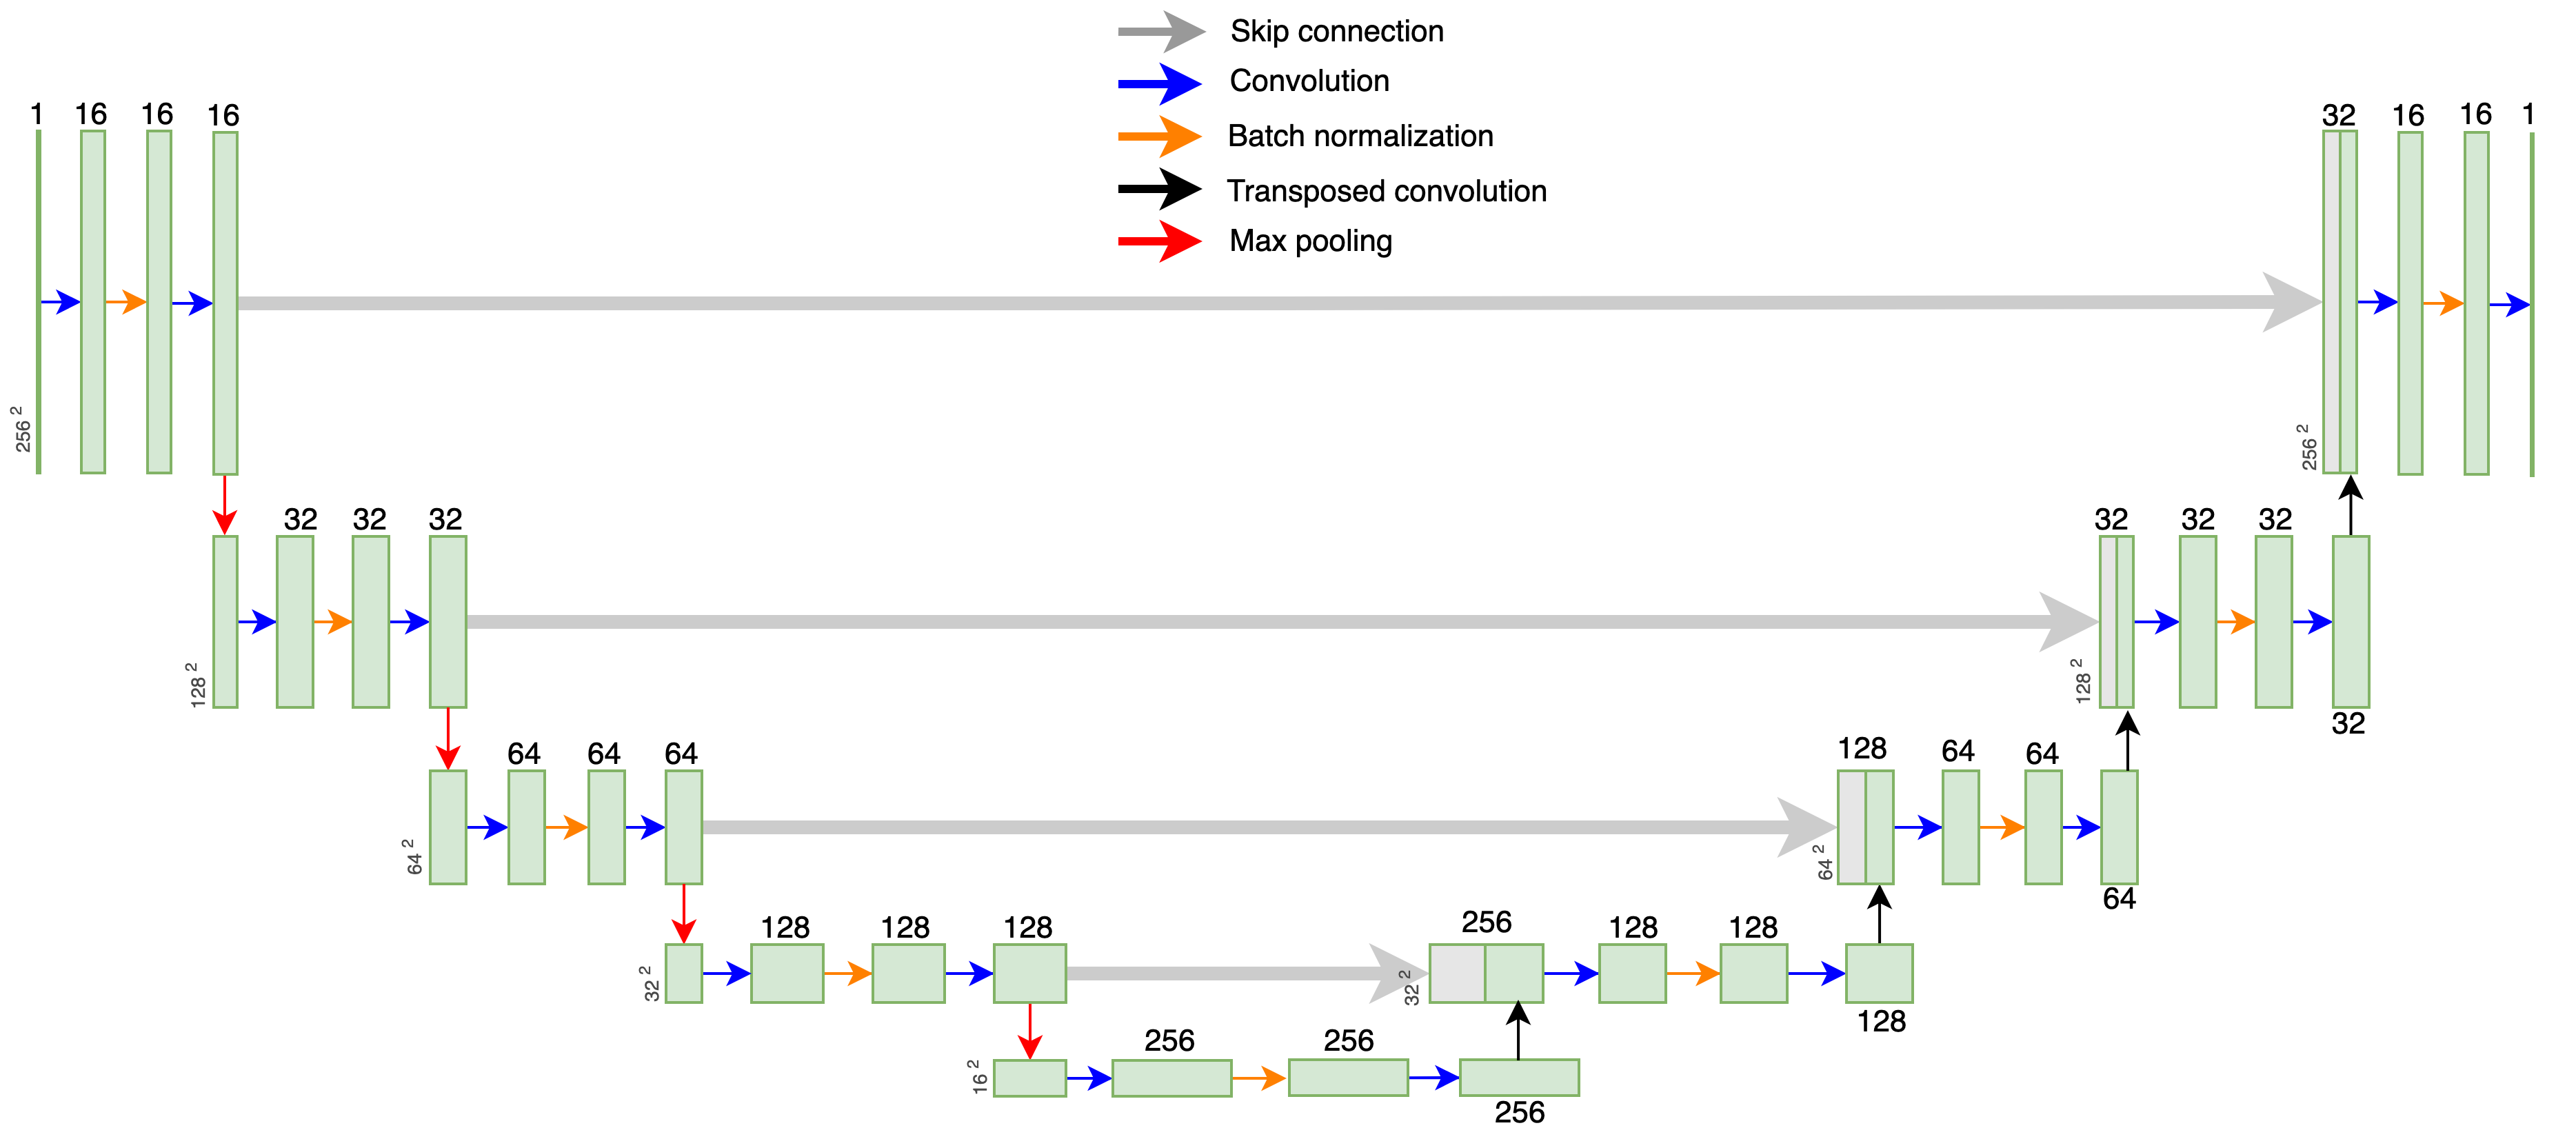
\includegraphics[width=\linewidth]{bilder/Unet.png}
		\caption{Unet}\label{fig:unet}
	\end{center}
\end{figure}
